\input{../header}
\usepackage{pgfplots}
\rhead{Your name: \rule{8cm}{0.15mm}}

\everymath{\displaystyle}
\begin{document}
%


%\onehalfspacing
\allowdisplaybreaks
%##################################################################
\section{Chapter 4 checkpoint!}

Chapter 1 scorecard:
\begin{center}
    \begin{tabular}{|m{3.75cm}|*{5}{m{2cm}|}} \hline
        Learning target: & DF1 & DF2 & DFa & DFb & AD2 \\\hline
        Your confidence level before starting (0-5): & &&&&\\\hline
        Your confidence level after the quiz (0-5): & &&&&\\\hline
        The mark you earned on this attempt: 
        & Success! \newline Try again!
        & Success! \newline Try again!
        & Success! \newline Try again!
        & Success! \newline Try again!
        & Success! \newline Try again! \\\hline

    \end{tabular}
\end{center}
Chapter 2 scorecard:
\begin{center}
    \begin{tabular}{|m{3.75cm}|*{6}{m{2cm}|}} \hline
        Learning target: & DF3 & DF4 & DF5 & DF6 & DF7 \\\hline
        Your confidence level before starting (0-5): & &&&&\\\hline
        Your confidence level after the quiz (0-5):  & &&&&\\\hline
        The mark you earned on this attempt: 
        & Success! \newline Try again!
        & Success! \newline Try again!
        & Success! \newline Try again!
        & Success! \newline Try again!
        & Success! \newline Try again!\\\hline

    \end{tabular}
\end{center}

Chapter 3 scorecard:
\begin{center}
    \begin{tabular}{|m{3.75cm}|*{6}{m{2cm}|}} \hline
        Learning target: & AD3 & AD4 & AD5 & AD8 & AD9 \\\hline
        Your confidence level before starting (0-5): & &&&&\\\hline
        Your confidence level after the quiz (0-5):  & &&&&\\\hline
        The mark you earned on this attempt: 
        & Success! \newline Try again!
        & Success! \newline Try again!
        & Success! \newline Try again!
        & Success! \newline Try again!
        & Success! \newline Try again!\\\hline

    \end{tabular}
\end{center}

Chapter 4 scorecard:
\begin{center}
    \begin{tabular}{|m{3.75cm}|*{6}{m{2cm}|}} \hline
        Learning target: & IN1 & IN2 & IN3 & IN5 & INx \\\hline
        Your confidence level before starting (0-5): & &&&&\\\hline
        Your confidence level after the quiz (0-5):  & &&&&\\\hline
        The mark you earned on this attempt: 
        & Success! \newline Try again!
        & Success! \newline Try again!
        & Success! \newline Try again!
        & Success! \newline Try again!
        & Success! \newline Try again!\\\hline

    \end{tabular}
\end{center}


Have fun and do your best! I believe in u $\heartsuit$


%%%%%%%%%%%%%%%%%%%%%%%%%%%%%%%%%%%%%%%%%%%%%%%%%%%%%%%%%
\pagebreak
%%%%%%%%%%%%%%%%%%%%%%%%%%%%%%%%%%%%%%%%%%%%%%%%%%%%%%%%%
\providecommand{\stxKnowl}{}\renewcommand{\stxKnowl}[1]{#1 \vfill}
\providecommand{\stxOuttro}{}\renewcommand{\stxOuttro}[1]{#1}
\providecommand{\stxTitle}{}\renewcommand{\stxTitle}[1]{#1}
% Comment next line to show outtros
\renewcommand{\stxOuttro}[1]{}


\section{Learning target IN1, version 1}

Here is the graph of a function $h(t)$, which is made up of only straight lines and parts of circles.

\includegraphics[width=\textwidth]{../images/IN1-v1.png}

Compute each of the following.

\begin{multicols*}{2}
{\everymath{\displaystyle}
\begin{enumerate}[(a)]
    \item $\int_{-4}^0 h(t)\, dt$

    \vfill
    \item $\int_0^2 h(t)\, dt$

    \vfill
    \item $\int_2^4 h(t)\, dt$

    \vfill
    \item $\int_4^7 h(t)\, dt$

    \vfill
    \columnbreak
    \item $\int_7^8 h(t)\, dt$

    \vfill
    \item $\int_8^{9.2} h(t)\, dt$

    \vfill
    \item $\int_{9.2}^{10} h(t)\, dt$

    \vfill
    \item $\int_{-4}^{10} h(t)\, dt$

\end{enumerate}
}
\end{multicols*}
%%%%%%%%%%%%%%%%%%%%%%%%%%%%%%%%%%%%%%%%%%%%%%%%%%%%%%%%%
\pagebreak
%%%%%%%%%%%%%%%%%%%%%%%%%%%%%%%%%%%%%%%%%%%%%%%%%%%%%%%%%

\section{Learning target IN2 and INx, version 1}

The rate at which pollution escapes a scrubbing process at a manufacturing plant increases over time as filters and other technologies become less effective. Suppose that the rate of pollution (measured in tons per week) is given by the function $r$ that is pictured below. Throughout this problem, we're interested in $\displaystyle\int_{t=0}^5 r(t)\, dt$.

\includegraphics[width=0.5\textwidth]{../images/IN2-v1.png}
\includegraphics[width=0.5\textwidth]{../images/IN2-v1.png}
\begin{enumerate}[(a)]
\item On the first graph above, carefully draw the \textit{left} Riemann sum with four rectagles of uniform width. (How wide should each rectangle be?)
\item On the second graph above, carefully draw the \textit{right} Riemann sum with four rectangles.
\item If $r(t) = 0.5 e^{0.5t}$, compute both of these Riemann sums. Show your work for computing the heights of the rectangles. (Hint: lots of your work will overlap!)

\textbf{Include units on every number you write.}
\vfill
\item Give your best guess for $\displaystyle\int_{t=0}^5 r(t)\, dt$, \textbf{include units}, and explain what this number means about pollution.
\end{enumerate}

\iffalse
\section{Learning target IN2, version 2}

Here is a graph of the function $f(x) = 4x^2 - 6x^3 + 9x$ on the interval $[0, 2]$.

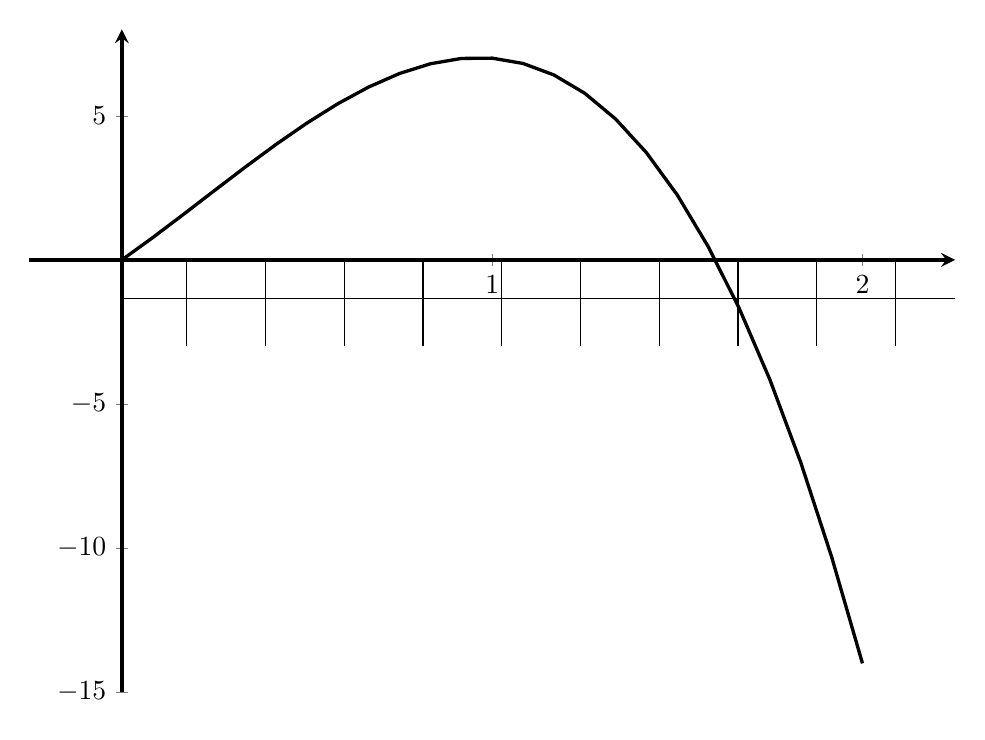
\begin{tikzpicture}
    \begin{axis}[
        width=1.1\textwidth, height=10cm,
        xmin=-0.25, xmax=2.25, ymin=-15, ymax=8,
        xtick distance = 1, ytick distance = 5,
        minor x tick num = 0, minor y tick num = 0,
        xticklabel style={anchor=north},
        yticklabel style={anchor=east},
        major grid style={thin, black!50},
        grid=none, 
        axis lines=center, axis line style = very thick]
        \draw (0,0) grid (3, -3);
        \addplot[very thick, domain=0:2] {4*x^2 - 6*x^3 + 9*x };
    \end{axis}
\end{tikzpicture}

\begin{enumerate}[(a)]
    \item \textit{Without computing it,} would you guess that $\displaystyle\int_0^2 f(x)\ dx$ is positive or negative? Why?
    \item Let's use a \textit{right} Riemann sum with 6 rectangles of uniform width to approximate $\displaystyle\int_0^2 f(x)\ dx$.

    Draw the six rectangles on the graph above.
    \item How wide should each rectangle be?
    \vfill
    \item Compute the right Riemann sum. Show your work to find the height of each rectangle.
    \vfill
    \vfill
\end{enumerate}
\fi

%%%%%%%%%%%%%%%%%%%%%%%%%%%%%%%%%%%%%%%%%%%%%%%%%%%%%%%%%
\pagebreak
%%%%%%%%%%%%%%%%%%%%%%%%%%%%%%%%%%%%%%%%%%%%%%%%%%%%%%%%%

\section{Learning target IN3, version 1} % checkit 18, modified

\stxKnowl{
 Explain how to find the \textit{general} antiderivative for each function. 
 
 (Hint: Derivatives eat constants, so what should antiderivatives do?)

\begin{enumerate}[(a)]
\item
\stxKnowl{
\( 2^x + 3^x - 5^x \)

\stxOuttro{
\[\renewcommand{\log}{\ln}\frac{1}{\cos\left(x\right)}+C\]

}
}

\item
\stxKnowl{
\(\renewcommand{\log}{\ln}7 \, x^{4} + 4 \, x^{3} - x\)

\stxOuttro{
\[\renewcommand{\log}{\ln}\frac{7}{5} \, x^{5} + x^{4} - \frac{1}{2} \, x^{2}+C\]

}
}

\item
\stxKnowl{
\(\renewcommand{\log}{\ln}5 \, \sin\left(x\right)\)

\stxOuttro{
\[\renewcommand{\log}{\ln}-5 \, \cos\left(x\right)+C\]

}
}

\item
\stxKnowl{
\(\renewcommand{\log}{\ln}\frac{1}{5 \, x^{1/5}}\)

\stxOuttro{
\[\renewcommand{\log}{\ln}\frac{1}{4} \, x^{\frac{4}{5}}+C\]

}
}

\end{enumerate}
}

%%%%%%%%%%%%%%%%%%%%%%%%%%%%%%%%%%%%%%%%%%%%%%%%%%%%%%%%%
\pagebreak
%%%%%%%%%%%%%%%%%%%%%%%%%%%%%%%%%%%%%%%%%%%%%%%%%%%%%%%%%

\section{Learning target IN5, version 1} % checkit 15

\stxKnowl{
 Explain how to compute the exact value of each of the following definite integrals using the Fundamental Theorem of Calculus. 
 
 \textbf{Leave all answers in exact form, with no decimal approximations. }

\begin{enumerate}[(a)]
\item
\stxKnowl{
 \(\displaystyle \int_{ x=4 }^{ 6 } \left( \frac{6}{x} \right) dx\) 

\stxOuttro{
\[-6 \, \log\left(6\right) + 12 \, \log\left(2\right)\]

}
}

\item
\stxKnowl{
 \(\int_{x= \frac{5}{4} \, \pi }^{ \frac{4}{3} \, \pi } \left( -2 \, \sec^2\left(x\right) \right) dx\)

\stxOuttro{
\[-2 \, \sqrt{3} + 2\]

}
}

\item
\stxKnowl{
 \(\int_{x= -2 }^{ -1 } \left( 3 \, x^{3} + 10 \, x - 1 \right) dx\)

\stxOuttro{
\[-\frac{109}{4}\]
}
}

\end{enumerate}
}


\end{document}